% vim: set spelllang=fr:

\setchapterpreamble[ur][.5\textwidth]{%
  \dictum[Robin Hobb, \textit{Assassin's Quest}]{%
As for me, I had been amazed at how many pieces there were to something that had seemed to be all one thing when I had started in on it. [...] All these sounds to make a word, all these words to frame a thought. Language came apart in my hands. I had never stopped to consider it before.}}

\chapter{État de l'art} 
\label{ch:etatdelart} 
% TODO Questions :
%   - inventaires vs. inventaires de sens
%   - qui citer pour sème ?
%   - qui citer pour plus d'un sens ?
%   - réutiliser la figure d'un papier ?


La représentation du sens des mots (section~\ref{sec:mots}) occupe une place
importante dans nos travaux, en particulier pour la traduction de la ressource
WordNet (Chapitre~\ref{ch:wonef}). La traduction de ressources lexicales
(section~\ref{sec:translation}) est un moyen de faire profiter une langue cible
de l'effort fourni pour une langue source, comme nous le faisons dans la
partie~\ref{part:translation}. Enfin, l'annotation en rôles sémantiques
(section~\ref{sec:srl}) sera elle surtout utile pour la partie~\ref{part:srl}.

\section{Représentation des mots}
\label{sec:mots}

% TODO \citep{harnad1990symbol} ?
Nous étudions ici différentes façons de représenter les mots et leur sens en
commençant par les dictionnaires, puis en étudiant différentes ressources
lexicales représentant le sens des mots. Enfin, nous présentons les modèles de
langue qui sont une manière plus directe de représenter les mots à partir d'un
corpus.

\subsection{Représentation du sens des mots}
\label{subsec:sens_mots}

La lexicographie est la science qui consiste à recenser les mots, les classer,
les définir et les illustrer, par des exemples ou des expressions, pour rendre
compte de l'ensemble de leurs significations et de leurs acceptions au sein
d'une langue, afin de constituer un dictionnaire
\citep{wikipedia2014lexicographie}. La lexicographie est donc un socle sur
lequel le Traitement Automatique des Langues peut s'appuyer pour représenter le
sens des mots.

Pour pouvoir identifier les différents sens d'un mot, les lexicographes
n'opèrent pas par intuition linguistique \citep{kilgarriff1997don}. Ils
commencent par établir un corpus équilibré et de taille assez importante pour
représenter la langue étudiée. Ce corpus peut par exemple être constitué de
textes de journaux, de fiction, ou encore de blogs, le tout étant supposé être
représentatif de ce qu'une personne lambda lit durant sa vie. Pour un mot
donné, le lexicographe examine ses différents usages dans ce corpus dans le but
de séparer ces différents usages en sens. Certains sens, jugés trop peu
fréquents, sont laissés de côté. Une fois la séparation effectuée, le
lexicographe l'étudie pour établir des critères objectifs distinguer les
différents sens du mot étudié. Une phase d'ajustement de la séparation suit
pour vérifier que les critères ont été correctement appliqués, ce qui peut
amener à raffiner ces critères. Une fois le processus fini, ces critères
serviront pour écrire la définition, et les occurrences de mots dans le corpus
pourront servir d'exemples. L'avantage principal est que le processus
lexicographique est désormais basé sur des données réelles et non pas sur des
intuitions linguistiques.

% exemple

Ainsi, les sens ne sont pas définis en tant que tels, mais sont avant tout des
occurrences dans un contexte donné. C'est une façon de comprendre la citation
de \citep{firth1957synopsys} : \emph{You shall know a word by the company it
keeps}\footnote{Vous devriez connaître un mot par ce qui l'accompagne.}. En
effet, selon \citep{kilgarriff1997don}, un ensemble de sens n'est défini que
par rapport à un corpus, et il est illusoire de vouloir définir un dictionnaire
parfait pour tous les sens possibles d'un mot.  Néanmoins, il n'est pas
concevable de réaliser manuellement un dictionnaire par corpus ; et il faut
simplement être conscient des difficultés théoriques posées par le sens des
mots.

Sans s'attarder sur des difficultés théoriques, on considèrera dans ce travail
que les sens définis dans un dictionnaire classique relèvent du «~domaine
général~», et que les sens qui apparaissent dans d'autres domaines sont des
sens «~spécialisés~». Par exemple, le dictionnaire DicoInfo \citep{corpusolst}
spécialisé dans les domaines de l'Informatique et d'Internet mentionne un sens
spécifique pour le nom \emph{compilation} : \emph{action effectuée par un
compilateur qui consiste à transformer du code créé au moyen d'un langage de
programmation évolué en un langage compréhensible par l'ordinateur}. Ce sens
est par exemple absent du TLFi \citep{TLFi} parce qu'il ne faisait pas partie
des sens du mot dans le corpus utilisé pour établir les définitions.

L'avènement de l'informatique a rendu possible d'autres moyen de représenter le
sens des mots. La qualité du travail lexicographique exposé dans les
dictionnaires n'a pas été remise en cause, mais :

\begin{itemize}

    \item les dictionnaires traditionnels, même dans leur version en ligne, ne
        tirent pas profit des nouveaux moyen d'organisation rendus possibles
        avec un ordinateur : il n'est plus nécessaire de trier les mots, on
        peut les représenter par un graphe
        \citep{miller1990introduction,polguere2013tissage},

    \item les dictionnaires traditionnels sont basés sur l'histoire des mots au
        lieu de considérer les progrès en linguistique et psycholinguistique
        proposant des organisations plus utiles et plus proches du lexique
        mental \citep{miller1990introduction}.

\end{itemize}

De plus, l'utilisation de dictionnaires récents implique un coût d'achat et le
respect de la licence restrictive, ce qui explique que ces dictionnaires ont
rapidement étés abandonnés en TAL au profit d'autres ressources disponibles
sous une licence libre comme WordNet \citep{fellbaum1998wordnet} ou le
Wiktionnaire \citep{mouton2010jaws,nguyen2012using}. En effet, ces deux
ressources autorisent une utilisation à la fois à des fins de recherche mais
aussi pour un usage commercial, ce qui leur a assuré une large diffusion.

\subsection{WordNet}

% TODO étendre avec ce qui est dans jaws_translation_process et l'intro de
% ch:wonef

La première ressource lexicale à tirer partie de la possibilité de représenter
le lexique sous la forme d'un graphe est WordNet, dont l'élaboration a commencé
en 1985 \citep{miller1990introduction}. Établi sur des principes
psycholinguistiques, WordNet propose quatre graphes pour les quatre parties du
discours formant une classe ouverte : noms, verbes, adjectifs, adverbes. Les
nœuds du graphe sont des ensembles de synonymes (\emph{synonym sets} ou
\emph{synsets}). Un synset regroupe plusieurs mots, une définition, et
potentiellement des exemples.

\begin{figure}[h!]
    \centering
    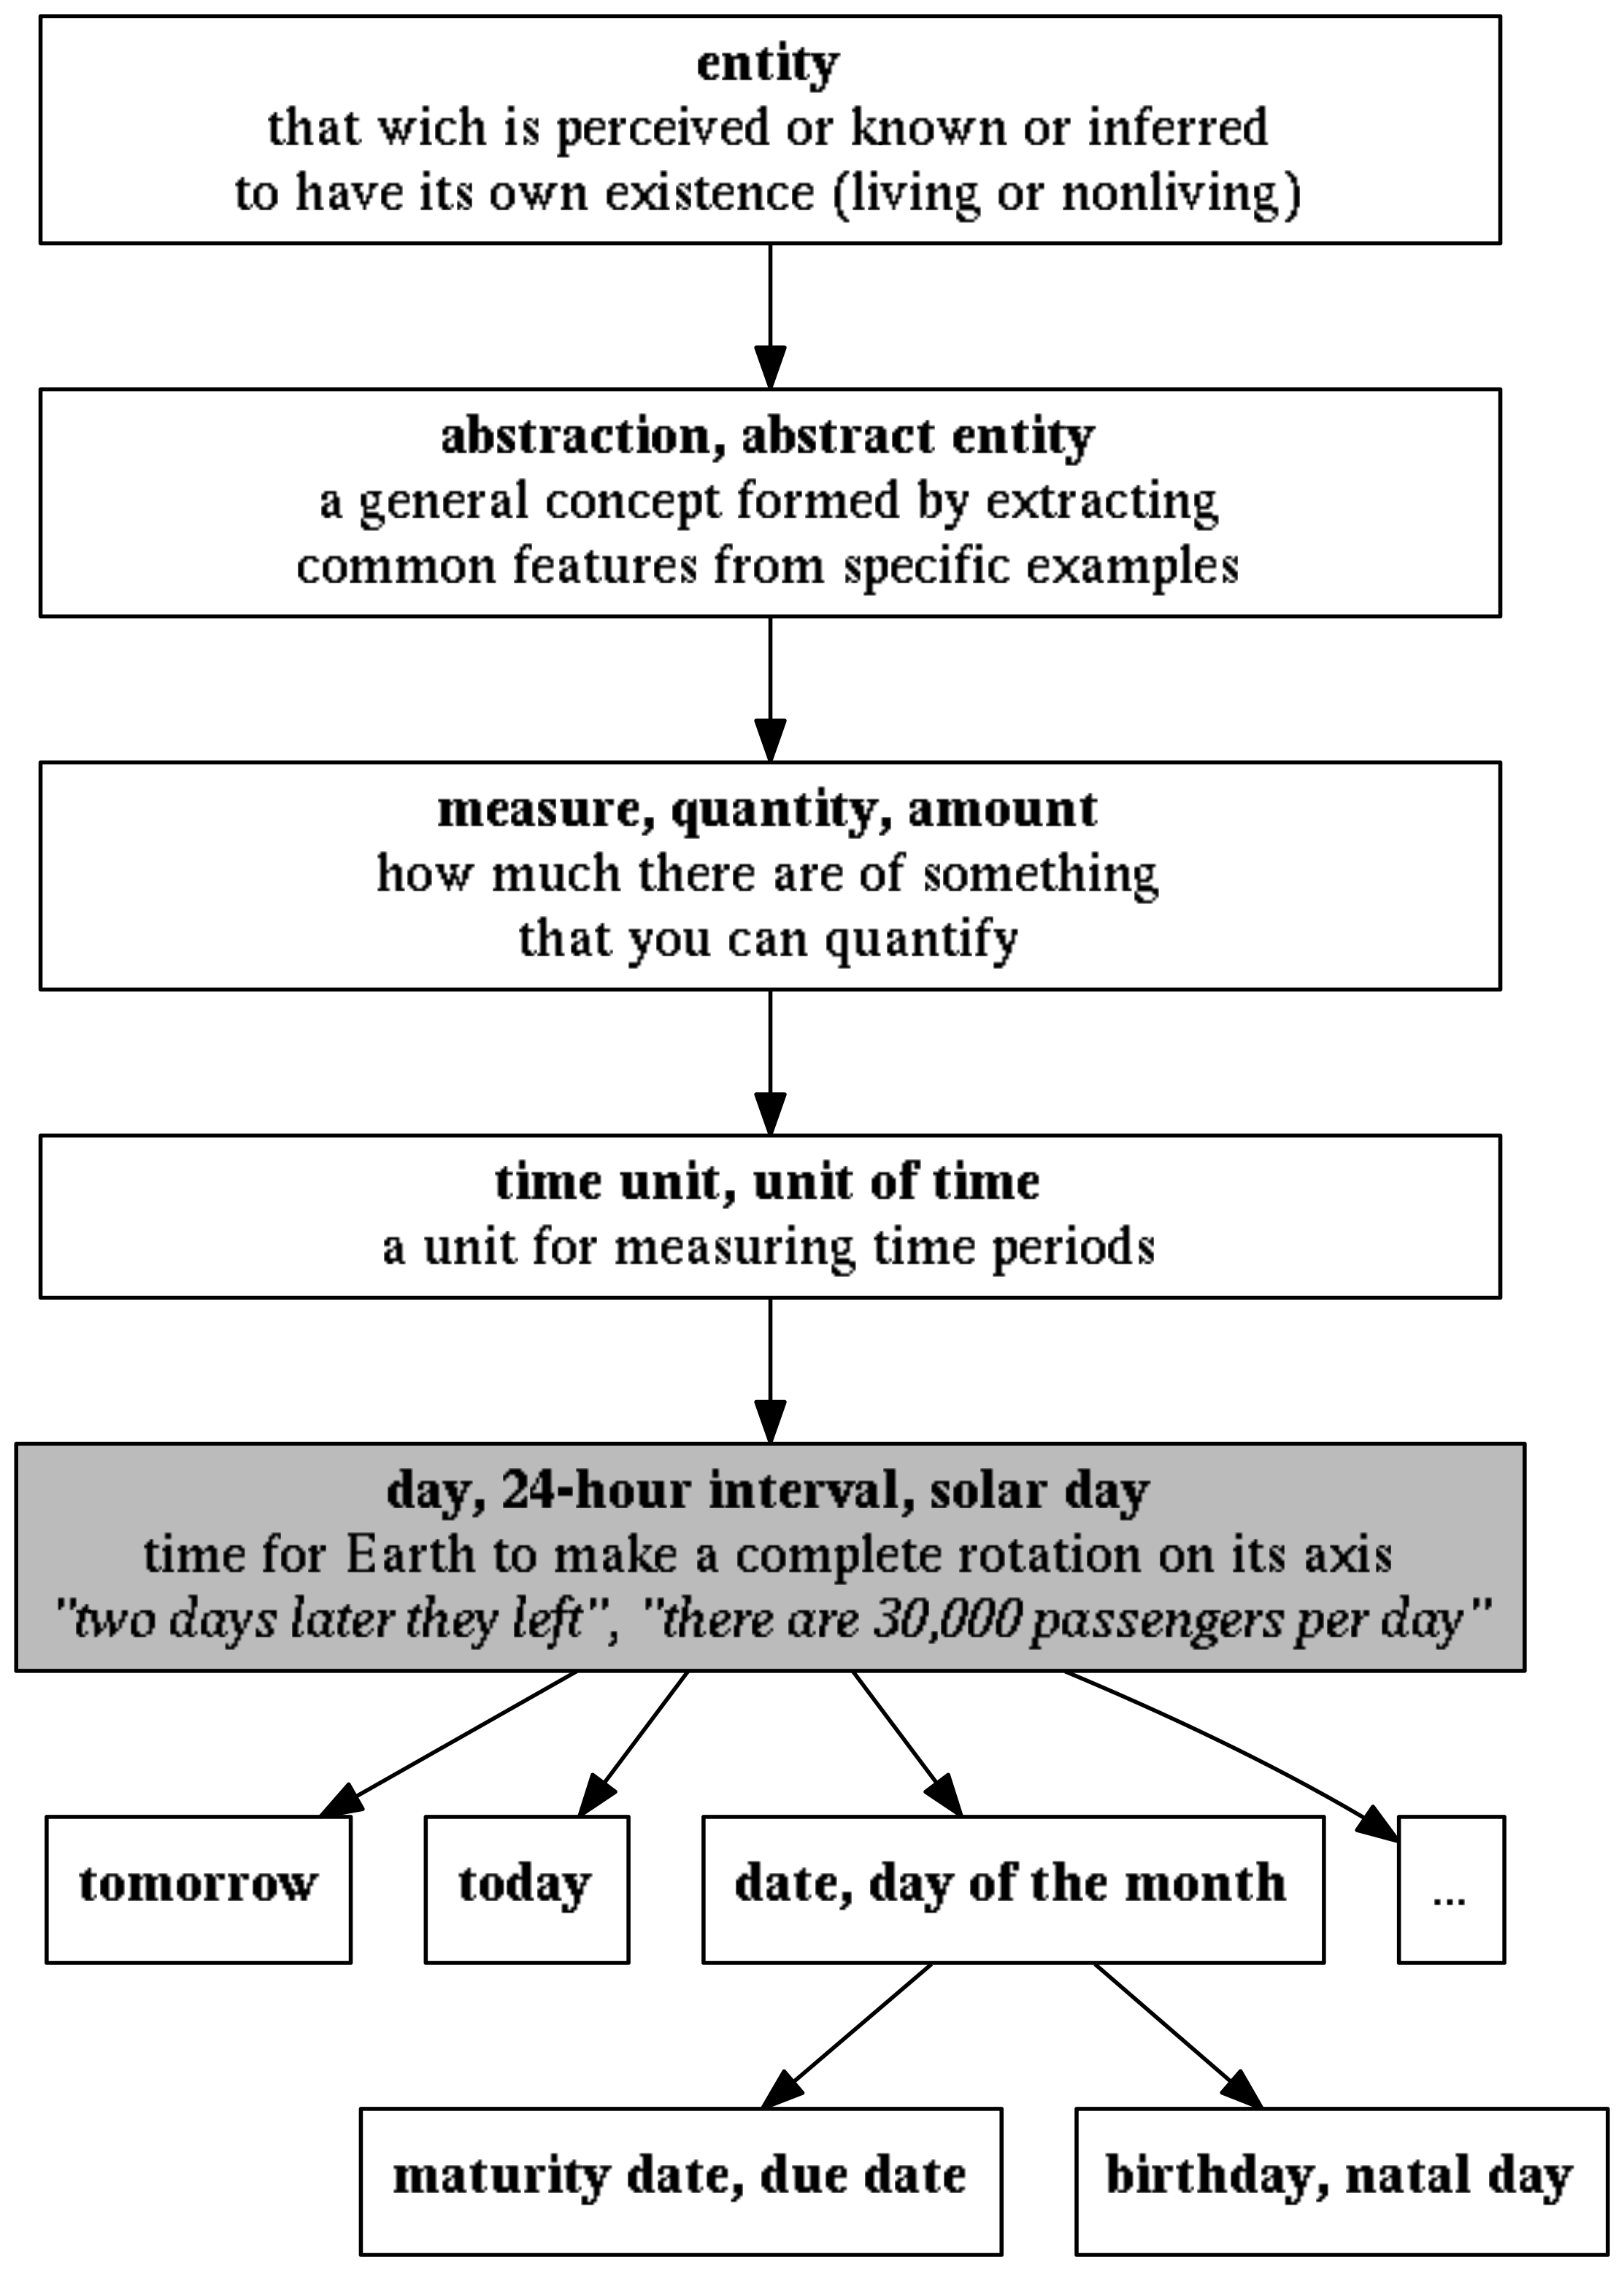
\includegraphics[width=0.7\textwidth]{fig/wordnet_hypernymy.png}
    \caption{\label{fig:wordnet_hypernymy}Hypéronymie dans WordNet autour du
        synset \emph{day}. Les synsets au-dessus de \emph{day} sont ses hypéronymes
        (\emph{day} est-un \emph{time unit}), et les synets au-dessus font partie de
        ses hyponymes (\emph{tomorrow} est-un \emph{day}).}
\end{figure}

\begin{figure}[h!]
    \centering
    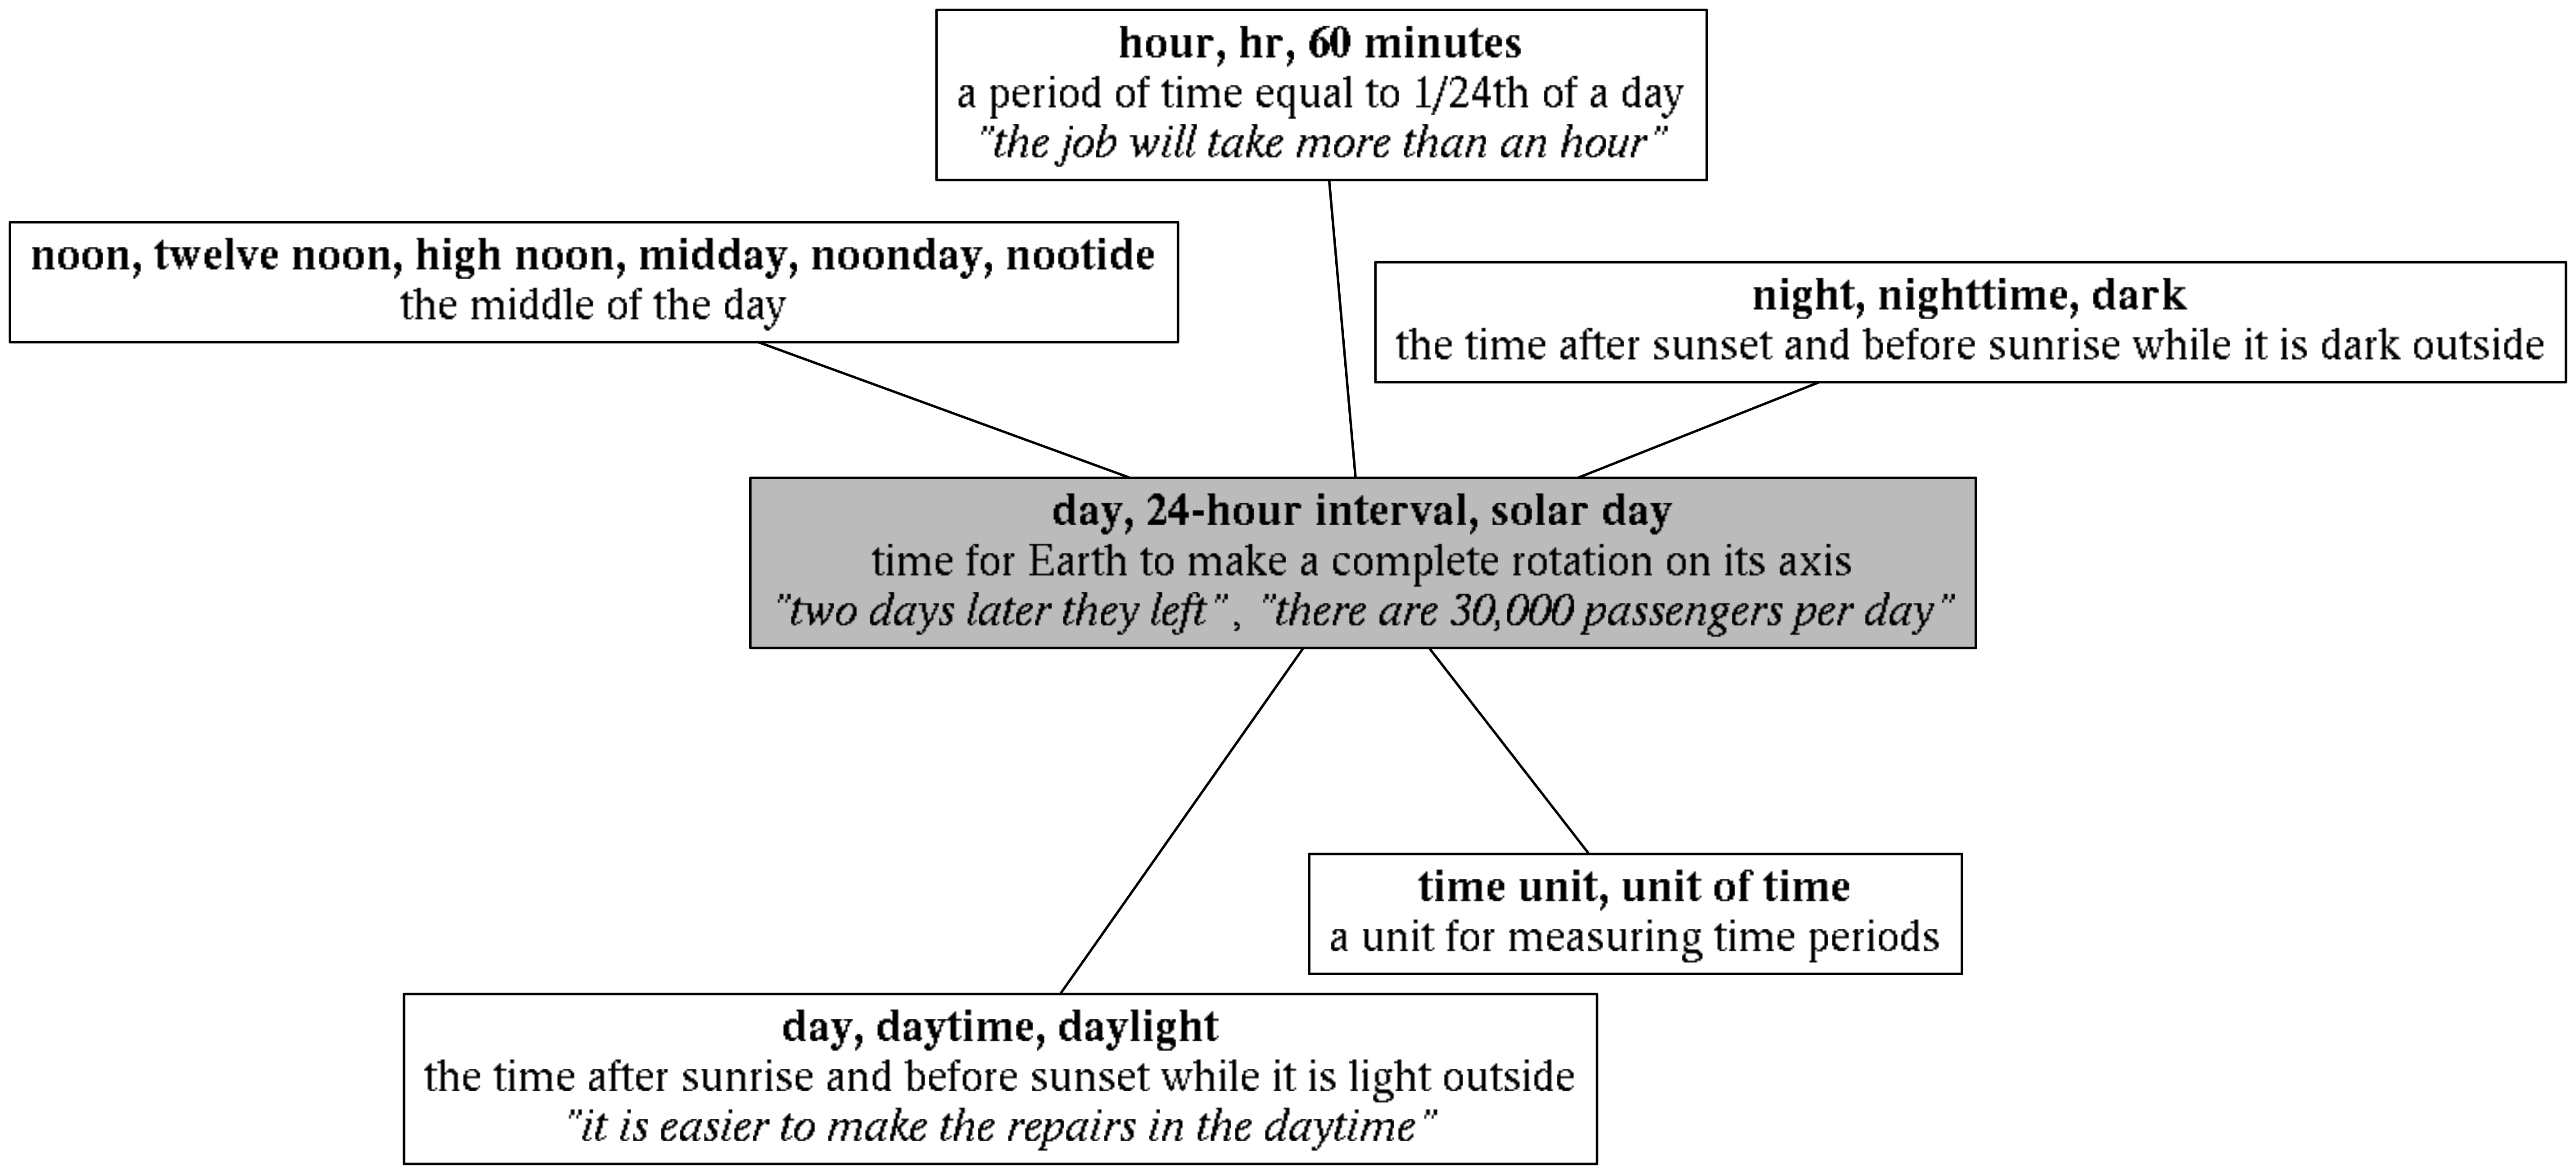
\includegraphics[width=0.9\textwidth]{fig/wordnet_relations.png}
    \caption{\label{fig:wordnet_relations} Le synset \emph{day} est aussi lié à
        d'autres synsets si on considère d'autres relations que l'hypéronymie et
        l'hyponymie.}
\end{figure}

Chaque synset est lié à d'autres synsets à travers un certain nombre de
relations telles que l'hypéronymie, la méronymie de partie (\emph{guidon} est
un méronyme de partie de \emph{vélo}), l'antonymie, etc. Si on ne considère que
l'hypéronymie, WordNet peut être visualisé comme un arbre
(Figure~\ref{fig:wordnet_hypernymy}). En considérant les autres relations,
WordNet est un graphe (Figure~\ref{fig:wordnet_relations}).

Les sens proposés ont étés utilisés pour annoter différents corpus dont le
corpus SemCor, ce qui a permis d'entraîner des systèmes supervisés. WordNet est
rapidement devenu le standard de la désambiguïsation lexicale et a été utilisé
dans de nombreuses campagnes d'évaluation \citep{navigli2009word}. C'est aussi
une ressource très utilisée de manière générale dans le domaine du Traitement
Automatique des Langues\footnote{Ses 10~000 citations sur Google Scholar au
moment de l'écriture de ce manuscrit sont le meilleur moyen de l'attester}.

\subsection{Autres inventaires de sens}

Depuis 2006, différents travaux \citep{hovy2006ontonotes,navigli2007semeval}
ont jugé que les défauts attribués à WordNet
\citep{boyd2006adding,ide2006making,snow2007learning} étaient suffisamment
importants pour nécessiter une alternative avec des sens distingués plus
grossièrement. Ce problème est attribué selon \cite{edmonds2002introduction} au
manque de rigueur lexicographique de WordNet, et à la mise en avant de la
similarité entre les mots à travers les synsets au détriment de la distinction
des sens. Il s'est en effet avéré que l'accord inter-annotateurs pour un
étiquetage avec WordNet est faible (de l'ordre de 70\%), et qu'utiliser un
autre inventaire un moyen efficace de s'adapter à différentes applications
\citep{palmer2004different}. La tendance est désormais à l'utilisation
d'inventaires plus grossiers \citep{navigli2007semeval,navigli2012quick}.

Au-delà des approches statistiques \citep{snow2007learning}, de nouveaux
inventaires de sens ont étés développés :

\begin{itemize}

    \item OntoNotes \citep{hovy2006ontonotes} a choisi de regrouper
        manuellement les sens WordNet jusqu'à obtenir un accord
        inter-annotateur de 90\%.

    \item DANTE\footnote{Les entrées pour les mots entre M et R sont
        disponibles sur http://webdante.com/} \citep{mccarthy2010dante} est un
        inventaire entièrement nouveau, conçu dans l'objectif de corriger les
        erreurs faites avec WordNet\citep{kilgarriff2010detailed}.

    \item Le Réseau Lexical du Français\citep{gader2014lexicon} lie des sens de
        mots avec de nombreuses fonctions lexicales associés à un degré de
        confiance, le tout permettant de produire des articles de dictionnaires.

\end{itemize}

Ces inventaires semblent plus adaptés que WordNet pour la désambiguïsation
lexicale \citep{navigli2012quick}, mais ils ne sont pas encore disponibles ou
ne sont pas utilisables librement à des fins commerciales.

Une approche complètement différente est celle de la structure de qualia
\citep{johnston1996qualia} qui s'inscrit dans le contexte plus général du
lexique génératif introduit par \cite{pustejovsky1991generative} qui considère
qu'une approche énumérative n'est pas viable. Le sens d'un mot est alors défini
selon plusieurs aspects prédéfinis (constitution, rôles, facteurs impliqués
dans la création, etc.) qui peuvent se retrouver dans plusieurs mots. Par
exemple, un couteau contient une lame et sert à couper. Cette approche est
semblable à celle qui définit le sens d'un mot comme une simple suite de sèmes.

Enfin, différents travaux mentionnent la possibilité d'utiliser plus d'un sens
pour un mot donné. \cite{smith2011rumble} propose d'utiliser des distributions
de probabilité sur les différents sens possibles pour définir un sens précis
dans un corpus. \cite{erk2013measuring} montrent qu'un accord inter-annotateur
haut peut être obtenu en demandant aux annotateurs d'indiquer pour chaque sens
sa correspondance avec l'usage sur une échelle de 1 à 5. Dans SemCor, les
annotateurs pouvaient choisir plusieurs sens si besoin, mais seulement 0.3\%
des occurrences de SemCor sont étiquetées avec plus d'un sens. Une campagne
d'évaluation a eu lieu en 2013 à ce sujet \citep{jurgens2013semeval}.

\subsection{Modèles de langue pour la similarité sémantique}
\label{subsec:modeles_de_langue}

Un modèle de langue prédit la probabilité d'un mot étant donné son contexte
dans la phrase. C'est directement utile pour des tâches telles que la
traduction automatique ou la reconnaissance de la parole dans lesquelles un
modèle de langue favorisera des phrases plausibles globalement au lieu
d'étudier chaque mot individuellement.

Ce n'est pas l'utilisation que nous faisons des modèles de langues : ici,
l'objectif est d'obtenir des mesures de similarité sémantiques utiles pour
notre traduction de WordNet (Chapitre~\ref{ch:wonef}) et pour notre module de
similarité entre syntagmes pour l'annotation en rôles sémantiques
(Chapitre~\ref{ch:semantic}).

Quelle est l'intuition derrière l'utilisation des modèles de langue ?
L'hypothèse distributionnelle s'explique ainsi
\cite[p.~786]{harris1954distributional} :

\begin{quote} ... si l'on considère que le sens de deux mots ou morphèmes A et B
    diffère davantage que le sens de A et C, alors on observe souvent que les
    distributions de A et B diffèrent davantage que les distributions de A et C.
    Autrement dit, la différence de sens est corrélée à la différence de
    distribution. \end{quote}

Les modèles de langue sont un moyen d'étudier ces distributions de probabilité.
On peut étudier deux types de distributions différentes correspondant à deux
types de relations entre les mots \citep{sahlgren2008distributional} :

\begin{itemize}
    \item les relations syntagmatiques identifient les mots qui sont présents
        ensemble dans un contexte donné ;
    \item les relations paradigmatiques identifient les mots qui sont présents
        dans un même contexte, mais sans y être présents ensemble.
\end{itemize}

Par exemple, étant donné les deux phrases \emph{Je bois du café} et \emph{Je
bois du thé}, on peut déduire que les lemmes \emph{boire} et \emph{thé} sont
liés par une relation syntagmatique : ils sont présents ensemble dans la
phrase. Au contraire, \emph{thé} et \emph{café} ne sont pas ici présents dans
la même phrase, mais apparaissent dans un même contexte (\emph{Je bois du}) :
ils sont liés par une relation paradigmatique.

Observer les distributions de contexte entre les mots permet à la fois
d'évaluer la similarité entre deux mots mais est aussi l'occasion de séparer
les mots suivant leurs sens \citep{yarowsky1993one,pantel2002discovering}. Un modèle de langue brut ne décrit que des lexèmes Nous
serons par la suite essentiellement concernés par les lexèmes : c'est-à-dire la
similarité entre les paires (lemme, sens) mais un modèle de langue ne peut
directement manipuler que des mots : la séparation se fait par la suite.

% \cite{schutze1998automatic,pantel2002discovering,niu2007three,pedersen2010duluth,liu2012semantic} ?

La question qui se pose maintenant que nous voulons observer les distributions
est : comment représenter et calculer ces distributions ? Une façon d'opérer
est de calculer la probabilité d'un mot dans une phrase étant donné les mots
précédents. Par exemple, étant donné le début de phrase "Au-delà des approches
...", on veut connaître la probabilité du mot suivant, en espérant que celle de
\emph{statistiques} ou \emph{supervisées} soit plus importante que celle de
\emph{chat}. En prenant par exemple le contexte des deux mots qui précèdent le
mot étudié, on calcule sa probabilité simplement avec le maximum de
vraisemblance :

\[
p(w_i|w_{i-2}, w_{i-1}) = \frac{compte(w_{i-2}, w_{i-1}, w_i)}{compte(w_{i-1}, w_i)}
\]

La séquence $w_{i-2}, w_{i-1}, w_{i}$ est un 3-gramme, et $compte$ compte le
nombre d'occurrences de cette séquence dans le corpus considéré. La taille du
contexte peut varier, ce qui est la raison pour laquelle on parle de manière
générale de n-grammes. Le nombre de paramètres à estimer pour obtenir une
distribution de probabilité conditionnelle fiable dépend de la taille du
vocabulaire ($|V|$) et de la taille du contexte étudié ($n$) et vaut $|V|^n$.
En considérant un petit vocabulaire (10~000 mots) et un contexte de trois mots,
il faut déjà estimer $10^{12}$ probabilités, ce qui requiert un corpus très
large : Google a utilisé un corpus de livres d'un trillion de mots pour estimer
ses n-grammes allant jusqu'à $n=5$ \citep{brants2006web}. Diverses techniques
de lissage existent pour mieux répartir les probabilités
\citep[Chapitre~4]{jurafsky2008speech}. En effet, la plupart des probabilités
sont initialement nulles, que ce soit parce que le n-gramme est
grammaticalement invalide ou simplement parce qu'il n'a pas été observé dans le
corpus étudié. Il faut leur assigner une probabilité très faible afin d'éviter
de multiplier des probabilités nulles et de perdre ainsi de l'information.

Diverses extensions de ces modèles de langues à base de n-grammes existent,
l'une d'entre elles étant le modèle de langue syntaxique
\citep{lin1998automatic,goldberg2013dataset}. Dans ce modèle, on considère les
mots présents ensemble dans une relation syntaxique donnée. Pour la relation
complément du nom par exemple, on s'attend à ce que \emph{vélo} soit le
complément du nom des mots \emph{pédale}, \emph{guidon}, \emph{pneu} et ainsi
de suite. Le modèle de langue syntaxique que nous utilisons pour traduire
WordNet a été entraîné sur un corpus extrait du web francophone
\citep{grefenstette2007conquering}. Le corpus a ensuite été analysé par LIMA
\citep{besancon2010lima}, une chaîne d'analyse linguistique désormais libre ici
utilisée comme un analyseur syntaxique à base de règles produisant des
dépendances syntaxiques fines. Pour une relation donnée $r$ et un lemme $x$, le
modèle de langue indique quels sont les 100 premiers lemmes co-occurrant le
plus fréquemment avec $x$ dans la relation $r$.  Avec le mot \textit{avion} et
la relation de complément du nom, le mot \textit{billet} modifie le plus
\textit{avion} : \textit{billet d'avion} est fréquent dans le corpus. Ce modèle
de langue peut-être visualisé sur
\url{http://www.kalisteo.fr/demo/semanticmap/}.

D'autres types de modèles de langue représentent les mots de manières
distribuée en utilisant un vecteur de nombres réels. La manière la plus
répandue pour faire cela est d'utiliser un réseau de neurones dont une des
couches sera le vecteur représentant chaque mot. \cite{hinton1986learning} a
d'abord proposé l'idée d'un réseau de neurones pour représenter des concepts,
puis \cite{bengio2001neural,bengio2003neural} ont proposé le modèle de langue
neuronal tel qu'on le connaît aujourd'hui. Ce modèle de langue calcule non
seulement la probabilité d'un mot étant donné les mots précédents : c'est la
tâche sur laquelle il est entraîné. Mais il obtient aussi une représentation de
chaque mot où les mots sémantiquement proches ont des représentations proches.

% TODO LSA fait une partie du chemin
% TODO collobert & weston ? liens entre rns ?

\cite{mikolov2013efficient} et l'outil word2vec
associé\footnote{\url{https://code.google.com/p/word2vec/}} ont rendu possible
l'application de tels réseaux de neurones accessible et efficace. Une propriété
particulièrement intéressante des réseaux de neurones obtenus est que la
distance entre certains mots est fixe. En particulier, dans cet espace de
vecteurs :

\begin{itemize}
    \item reine + homme - femme = roi
    \item Paris - France + Spain = Madrid
    \item Australian - Australia + France = French
\end{itemize}

Ces résultats non prévus (la tâche était uniquement de prédire le mot en
fonction de son contexte) illustrent le type de généralisation obtenues à
l'aide d'un réseau de neurones et qui seraient autrement inaccessibles.

Ces réseaux de neurones sont encore difficiles à entraîner et à paramétrer
\citep{do2014modeles}, mais représentent une alternative bien plus efficace que
les modèles de langue simples à base de n-grammes parce qu'ils généralisent
bien mieux que la simple utilisation du maximum de vraisemblance
\citep{olah2014deep}.

% TODO donner des raisons de l'efficacité, "exponentiel" tout ça

\section{Traductions de ressources linguistiques}
\label{sec:translation}

\subsection{WordNet}

Les traductions automatiques de WordNet emploient une approche dite d'extension
(\textit{extend approach}) : la structure de WordNet est préservée et seuls les
littéraux sont traduits. Trois techniques principales représentent cette
approche dans la littérature. La plus simple utilise des dictionnaires
bilingues pour faciliter le travail des lexicographes qui filtrent ensuite
manuellement les entrées proposées
\citep{vossen1998eurowordnet,pianta2002developing,tufis2004balkanet}. Une
deuxième méthode de traduction utilise des corpus parallèles, ce qui évite
l'utilisation de dictionnaires qui peuvent entraîner un biais lexicographique.
\cite{dyvik2004translations} représente cette méthode en s'appuyant sur des
\textit{back-translations} entre le norvégien et l'anglais, alors que
\citep{sagot2008construction} combinent un lexique multilingue et les
différents WordNets de BalkaNet comme autant de sources aidant à la
désambiguïsation. Enfin, plus récemment, des ressources telles que Wikipédia ou
le Wiktionnaire ont été explorées. Grâce aux nombreux liens entre les
différentes langues de ces ressources, il est possible de créer de nouveaux
wordnets \citep{demelo2009towards,navigli2010babelnet} ou d'améliorer des
wordnets existants \citep{hanoka2012wordnet}.

Concernant le français, l'EuroWordNet \citep{vossen1998eurowordnet} est la
première traduction française de WordNet. C'est une ressource d'une couverture
limitée qui demande des améliorations significatives avant de pouvoir être
utilisée \citep{jacquin2006systemes}, et qui n'est ni libre ni librement
accessible. WOLF est une seconde traduction initialement construite à l'aide de
corpus parallèles \citep{sagot2008construction} et étendue depuis avec
différentes techniques \citep{apidianaki2012applying}. WOLF est distribué sous
une licence libre compatible avec la LGPL et c'est aujourd'hui le WordNet
français standard. Enfin, JAWS \citep{mouton2010jaws} est une traduction des
noms de WordNet développée à l'aide de dictionnaires bilingues et d'un modèle
de langue syntaxique.

\label{subsec:jaws_translation_process}

Pour notre traduction de WordNet nommée WoNeF (Chapitre~\ref{ch:wonef}), nous
reprenons les travaux de \cite{mouton2010jaws} qui ont abouti à JAWS, que nous
présentons ici. C'est un algorithme faiblement supervisé qui ne demande aucune
donnée annotée manuellement. Pour traduire un wordnet source, JAWS s'appuie sur
un dictionnaire bilingue et un modèle de langue syntaxique pour le langage
cible.

Le dictionnaire bilingue est une concaténation du dictionnaire bilingue
SCI-FRAN-EurADic\footnote{\url{http://catalog.elra.info/product_info.php?products_id=666}}
et des liens entre les Wiktionnaires français et
anglais\footnote{\url{http://www.wiktionary.org/}}. Le modèle de langue
syntaxique a été présenté à la section~\ref{subsec:modeles_de_langue}. Grâce
aux dictionnaires, JAWS n'a pas besoin de sélectionner les littéraux de chaque
synset parmi l'ensemble du vocabulaire mais seulement parmi un petit nombre de
candidats (9 en moyenne).  Le processus de traduction se fait en trois étapes :
\begin{enumerate} \item Créer un wordnet vide : la structure de WordNet est
préservée, mais les synsets eux-mêmes n'ont pas de littéraux associés.  \item
Choisir les traductions les plus faciles parmi les candidats des dictionnaires
pour commencer à remplir JAWS.  \item Étendre JAWS de manière incrémentale en
utilisant le modèle de langue, les relations entre synsets et le JAWS déjà
existant.  \end{enumerate}

\paragraph{Sélecteurs initiaux} Quatre algorithmes que nous nommons sélecteurs
initiaux choisissent des traductions correctes parmi celles qui sont proposées
par les dictionnaires. Premièrement, les mots qui apparaissent dans un seul
synset ne sont pas ambigus et il suffit d'ajouter toutes leurs traductions au
WordNet français : c'est le sélecteur par monosémie. C'est le cas de
\textit{grumpy} : toutes ses traductions sont validées dans le synset où il
apparaît. Deuxièmement, le sélecteur par unicité identifie les mots n'ayant
qu'une seule traduction et la valident dans tous les synsets où elle est
présente. Les cinq synsets contenant \textit{pill} en anglais sont ainsi
complétés avec \textit{pilule}. Un troisième sélecteur vise à traduire les mots
qui ne sont pas dans le dictionnaire en utilisant directement la traduction
anglaise : c'est le sélecteur des transfuges. Un quatrième sélecteur utilise la
distance d'édition de Levenshtein : si la distance entre un mot anglais et sa
traduction est petite, on peut considérer que c'est le même sens (c'est le cas
par exemple pour \textit{portion} ou encore \textit{university}), malgré
l'existence de certains faux amis. Ces quatre sélecteurs produisent une
première version du WordNet français qui contient assez de traductions pour
pouvoir ensuite utiliser le modèle de langue et continuer de compléter les
synsets.

\paragraph{Expansion de JAWS} JAWS étant partiellement rempli, une nouvelle étape d'expansion tire parti des relations entre les synsets de WordNet pour valider de nouvelles traductions. Par exemple, si :

\begin{itemize}
    \item un synset S1 est méronyme d'un synset S2 dans WordNet,
    \item il existe un contexte où un littéral dans S1 est méronyme d'un littéral candidat C dans S2,
\end{itemize}
alors ce littéral est considéré comme correct. La tâche de traduction est ainsi réduite à une tâche de comparaison entre d'une part les relations lexicales entre les synsets de WordNet et d'autre part les relations lexicales entre les lexèmes du français.

Prenons l'exemple de \textit{quill} qui peut se traduire par \textit{piquant} ou \textit{plume} (Figure \ref{meronymyexample}). Dans WordNet, \textit{quill} est méronyme de \textit{porcupine} qui a déjà été traduit par \textit{porc-épic} par un sélecteur initial. Dans le modèle de langue, \textit{piquant} fait partie des compléments du noms de \textit{porc-épic} mais ce n'est pas le cas de \textit{plume}. Ici, la relation de complément du nom implique la méronymie et c'est donc \textit{piquant} qu'il faut choisir comme la traduction correcte de \textit{quill}. Le modèle de langue a permis la désambiguïsation parmi les deux traductions possibles.

\tikzstyle{block}=[draw, fill=blue!5, rectangle, minimum height=0.5cm, minimum width=3cm, text width=5cm]

\begin{figure}[!ht]
  \centering
  \begin{tikzpicture}[auto, node distance=2cm,>=latex']
    % Inspired from http://www.texample.net/tikz/examples/control-system-principles/
    % first place and connect the outer blocks that represent synsets
      \node [block, text width=5cm] (quill) {~\\\textbf{Synset S1} \\ - Anglais : quill \\ - Français : piquant? plume? \\ (a stiff hollow protective spine on a porcupine) \\ ~ };
      \node [block, text width=4.0cm, right of=quill, node distance=9cm] (porcupine) {\textbf{Synset S2} \\ - Anglais : porcupine, hedgehog \\ - Français : porc-épic \\ (rodents with sharp erectile bristles mingled with the fur)};
    \draw [<-] (porcupine) -- node[above] {méronyme de} (quill);
    \draw [<-] (porcupine) -- node[below] {(relation WordNet)} (quill);

    % then the syntactic model relations
    \node [block, below of=porcupine, text width=4.0cm, node distance=3cm] (porcupinesynt1) {porc-épic};
    \node [block, below of=quill, node distance=3cm] (quillsynt1) {\Large{mémoire}, \Large{piquant}, \large{poil}, \large{épine}, yéti, ragoût, grotte, \small{tactique}, \small{pelage}, \small{dextre}, \small{aiguille}, ...};
    \draw [<-] (porcupinesynt1) -- node[above] {complément du nom de} (quillsynt1);
    \draw [<-] (porcupinesynt1) -- node[below] {(modèle de langue)} (quillsynt1);

  \end{tikzpicture}
  \caption{\protect\centering\label{meronymyexample}Traduction via la relation de méronymie de partie.}
\end{figure}

Un problème potentiel avec cette approche est que la relation de complément du nom n'est pas limitée à la méronymie. Par exemple, le mot \textit{mémoire} qui apparaît dans le modèle de langue vient d'un livre intitulé \textit{Mémoires d'un porc-épic}. Heureusement, \textit{mémoire} n'est pas dans les candidats de \textit{quill} et ne peut pas être choisi comme une traduction. Paradoxalement, le modèle de langue ne peut pas choisir entre deux mots très différents, mais est capable de choisir la traduction correcte d'un mot polysémique. Alors que traduire WordNet automatiquement avec un dictionnaire ou un modèle de langue syntaxique est impossible, combiner les deux ressources permet de résoudre le problème.

Chaque sélecteur suit le même principe que le sélecteur par méronymie de partie
et traduit de nouveaux synsets en identifiant les relations entre lexèmes via
le modèle de langue syntaxique. La correspondance entre la relation de
complément du nom et la relation de méronymie est directe, mais ce n'est pas le
cas pour les autres relations : il n'y a par exemple pas de relation syntaxique
qui exprime directement la synonymie entre deux lexèmes. Pour ces relations, il
est nécessaire d'employer soit des motifs lexicaux \citep{hearst1992automatic}
soit des relations syntaxiques de deuxième ordre \citep{lenci2012identifying}.
Ce sont ces dernières, aussi nommées relations paradigmatiques
(section~\ref{subsec:modeles_de_langue}, que JAWS utilise. Pour la synonymie,
si deux mots partagent les mêmes co-occurents dans une relation syntaxique
donnée, alors ils peuvent être synonymes dans ce contexte. Pour les noms, les
relations syntaxiques qui donnent les meilleurs résultats sont les relations de
complément du nom, d'objet du verbe et d'apposition. Concrètement, si deux noms
qui modifient les mêmes noms sont les objets des mêmes verbes ou sont apposés
aux mêmes noms, alors il est probable qu'ils soient synonymes et si l'un des
deux est déjà dans un synset, alors on peut y ajouter le second. Par exemple,
\textit{avant-propos} et \textit{préface} partagent les mêmes compléments du
noms : \textit{livre, édition, ouvrage}. Le sélecteur par synonymie peut
ajouter \textit{avant-propos} une fois que le littéral \textit{préface} est
dans JAWS. \citep{mouton2010jaws,mouton2010phd} décrivent d'autres sélecteurs
exploitant notamment les relations d'hyperonymie et d'hyponymie.

\subsection{VerbNet}
\label{subsec:presentation_verbnet}

\cite{levin1993english} est une classification des verbes anglais suivant un
principe simple : le comportement syntaxique des verbes détermine en partie
leur sens. Après avoir défini un certain nombre de constructions syntaxiques
possibles, les verbes sont classés en groupes partageant les mêmes
constructions. Le projet VerbNet a exporté les classes de Levin dans un format
électronique (XML) et a étendu la ressource avec de nouvelles classes,
constructions syntaxiques et verbes. VerbNet est une ressource lexicale pour
les verbes anglais organisée autour de classes sémantiques et de sous-classes
syntaxiques : une classe sémantique est divisée en sous-classes de verbes qui
partagent tous le même ensemble de cadres de sous-catégorisation
(Figure~\ref{fig:example_srl}, en suivant \cite{levin1993english}.  Dans sa
version actuelle\url{http://verbs.colorado.edu/~mpalmer/projects/verbnet.html},
VerbNet comprend 3769 lemmes, donnant lieu à 5257 entrées réparties en 274
sous-classes. VerbNet a montré la cohérence de sa classification et est très
utilisé, notamment pour l'annotation en rôles sémantiques
\citep{swier2005exploiting,palmer2013semantic} où il présente l'intérêt de ne
pas être restreint à un domaine spécifique tout en couvrant une large partie
des occurrences des verbes anglais dans un texte donné.

\begin{figure}[ht]
    \centering
    \begin{tabular}{ccc}
        \toprule
        Carol & crushed   & the ice \\
        Agent & V         & Patient \\
        \midrule
        The ice & crushes & easily  \\
        Patient & V       &         \\
        \bottomrule
    \end{tabular}
    \caption{\label{fig:example_srl}Ces deux phrases annotées avec la classe VerbNet carve-21.2 mettent en évidence que la position des arguments ne détermine pas directement les rôles: le sens et la voix de \textit{crush} ne change pas mais l'annotation sémantique est différente.}
\end{figure}

La traduction des classes de Levin et plus récemment de VerbNet dans d'autres
langue est une tâche reconnue comme utile dans la littérature. Initialement,
des méthodes automatiques ont mené à des améliorations dans le VerbNet anglais
lui-mmême après validation manuelle : de nouvelles classes ont été incorporées
\citep{korhonen2004extended} et de nouveaux verbes ont été ajouté à partir de
la base de données LCS \citep{dorr2001lcs} ou avec l'outil Sketch Engine
\citep{bonial2013expanding}. La base de données continue aujourd'hui d'évoluer,
la prochaine version prévue étant la 3.2.4.

Dans d'autres langues, \cite{merlo2002multilingual} ont utilisé des similarités
entres langues pour convertir 20 classes de Levin vers l'Italien. Des
acquisitions automatiques ont aussi été menées en japonais
\citep{suzuki2009classifying}, allemand \citep{im2006experiments} et espagnol
\citep{ferrer2004towards}. Les seules traductions directes dont nous avons la
connaissance sont le VerbNet estonien \citep{jentson2014verbnet} et le VerbNet
portuguais brésilien \citep{scarton2012towards} qui utilise des mappings entre
VerbNet et WordNet, et entre WordNet.Br et WordNet.

Pour le français, \cite{saintdizier1996constructing} a d'abord produit une
ressource proche des classes de Levin. À notre connaissance, l'effort sur cette
ressource a arrêté et le résultat n'est pas disponible. Des travaux se sont
ensuite concentrés sur l'acquisition automatique de cadres de
sous-catégorisation et sur le regroupement de verbes en se basant sur ces
cadres et sur des similarités sémantiques. \cite{sun2010investigating} ont
utilisé un large lexique de cadres de sous-catégorisation
\citep{messiant2010acquisition} pour regrouper les verbes en clusters à l'aide
de traits sémantiques (colocations et préférences lexicales des verbes) et
syntaxiques (cadres de sous-catégorisation). L'évaluation sur une
vérité-terrain créé manuellement a mené à une F-mesure de 55.1\%.
\cite{falk2012classifying} appliquent un algorithme de clustering différent et
utilisent des features différentes, ce qui améliore la F-mesure sur la même
vérité-terrain mais simplifiée. Ces ressources mettent en valeur de nouvelles
façons de séparer les verbes du Français, mais les erreurs qu'elles contiennent
seront une nouvelle source d'erreur dans les applications : il est important de
les corriger si possible.


\section{Annotation en rôles sémantiques}
\label{sec:srl}

Nous étudions les différentes façon de définir les rôles sémantiques, examinons
diverses ressources utiles pour la tâche d'annotation, et présentons diverses
techniques pour réaliser l'annotation elle-même.

\subsection{Les rôles sémantiques}
\label{subsec:roles_semantiques}

Comment aller au-delà d'une analyse syntaxique pour représenter le sens d'une
phrase ? La notion de rôle sémantique semble particulièrement adaptée aux
approches statistiques que nous présentons ici. Ces rôles ont pour objectif de
s'abstraire des alternances de diathèse présentes dans le langage naturel
(Figure~\ref{fig:example_srl}). Différentes théories linguistiques proposent
différentes représentations pour ces rôles ; nous nous intéresserons ici aux
rôles VerbNet et à la théorie élaborée par \cite{fillmore1968case} qui établit
que le cas grammatical exhibe des relations profondes et sémantiques. De
nombreuses langues marquent ces relations au niveau morphologique ; l'élatif
est un exemple de cas grammatical qui exprime le lieu de l'intérieur duquel
provient un mouvement et qui est marqué morphologiquement en finnois, hongrois
et estonien. Il est alors sensé de prévoir un rôle sémantique pour ce cas
grammatical, même s'il n'est pas marqué au niveau morphologique dans la langue
étudiée.

Il n'y a pas de réel consensus sur un inventaire de cas donnés. Parmi les rôles
sémantiques généralement acceptés, on peut citer :

\begin{itemize}
    \item l'\textbf{Agent} qui est à l'origine de l'action
    \item le \textbf{Patient} qui subit un changement d'état
    \item l'\textbf{Instrument} utilisé pour réaliser l'action
    \item le \textbf{Bénéficiaire} qui tire profit de l'action
\end{itemize}

\subsection{Lexiques et corpus}

Il existe en anglais différentes ressources pour l'annotation en rôles
sémantique : nous aborderons ici FrameNet, PropBank et NomBank, VerbNet ayant
déjà été présenté plus longuement à la
section~\ref{subsec:presentation_verbnet}. 

\paragraph{FrameNet}

FrameNet repose sur la théorie des \textit{Frame Semantics}, élaborée par
Fillmore en modifiant sa théorie initiale. Ici, les rôles sémantiques
\textit{frame elements} sont spécifiques à chaque situation (\textit{frame})
tout en se recoupant par endroits. On retrouve ainsi le rôle d'agent, mais
aussi des rôles spécifiques comme \textbf{Food} dans \textbf{Apply\_heat} ou
\textbf{Completeness} dans \textbf{Activity\_pause}. Les rôles sont classifiés
selon leur importance dans la situation : centraux (nécessaires), périphériques
(toujours liés à la situation mais optionnels) et circonstanciels
(potentiellement présent dans toutes les situations, par exemple le lieu ou le
temps).

\paragraph{PropBank}

Malgré quelques critiques \citep{riemer2011conception}, l'interface
syntaxe-sémantique nous permet d'utiliser les informations syntaxiques d'un
verbe pour distinguer différents sens et identifer ses arguments sémantique.
Par exemple, nous pouvons expliquer la différence entre deux sens majeurs du
verbe « retenir » ainsi :

\begin{enumerate}
    \item se souvenir de quelque chose
    \item empêcher quelqu'un de faire quelque chose
\end{enumerate}

PropBank \citep{palmer2005proposition} a décidé d'utiliser les annotations
syntaxiques du Penn TreeBank \citep{marcus1993building} pour annoter en rôles
sémantiques les phrases incluant un des 5000 verbes les plus fréquents du
corpus. Pour chaque phrase, les annotateurs ont identifié les syntagmes jouant
un rôles sémantique. L'objectif principal de PropBank est de permettre
d'utiliser l'apprentissage automatique pour l'annotation en rôles sémantiques.
C'est pour cette raison que les étiquettes disponibles sont très générales.
Ainsi, il est fréquent que \textit{ARG0} désigne l'agent, \textit{ARG1} le
patient. D'autres arguments sont disponibles pour étiqueter des rôles plus
spécifiques (\textit{ARG2}, \textit{ARG3}, etc.) ainsi que des rôles
secondaires (\textit{Location}, \textit{Extent}, \textit{Manner}, etc.)

\paragraph{NomBank}

NomBank \citep{meyers2004nombank} a été conçu à l'image de PropBank mais se
concentre, comme son nom l'indique, sur les noms communs, plus particulièrement
sur les 5 000 noms communs les plus fréquents dans le Penn TreeBank. Sur le
million de mots présent dans le corpus, 250 000 sont des noms communs. 100 000
d'entre eux sont des noms issus d'un verbe ou qui se comportent à la façon d'un
verbe. Par exemple, le nom commun français « achat » est lié au verbe « acheter
», et les arguments sémantiques seront probablement les mêmes : dans « Il a
acheté un arbre » et « l'achat d'un arbre », \textit{ARG1} sera dans les deux
cas l'arbre. D'autres catégories incluent les noms partitifs, relationnels et
environnementaux.

Pour une phrase telle que « They gave the chefs a standing ovation », les
annotations PropBank et NomBank peuvent montrer les liens possibles entre ces
deux ressources. Cette similarité volontaire a permis de lier ces ressources
\citep{pustejovsky2005merging,verhagen2007combining}, mais des applications
utilisant de telles ressources unifiées doivent encore voir le jour.

\cite{gerber2010beyond} ont étendu NomBank aux arguments
implicites, améliorant ainsi la couverture de NomBank de 65\%, c'est-à-dire en
augmentant le nombre moyen de rôles remplis dans chaque exemple annoté. Il
n'est pas rare que les arguments soient implicites mais présent dans d'autres
phrases. Les annotations étant limitées à la phrase actuelle, il n'est pas
possible de référer à un argument présent dans une prase précédente.

% TODO new PropBank LREC 2014

\subsection{Approches d'annotation}

Existing approaches to semantic role labeling are divided into two main
branches. The first one, supervised semantic role labeling, uses a
manually-annotated corpus and manually engineered features to train supervised
models on the task. The most used frame-semantics resource and associated
annotated corpus in this domain is FrameNet \citep{baker1998berkeley}.
While this approach yields the best performance \citep{das2014frame}, the
cost is high: the corpus used are annotated over several years and it would be
in general too long and costly to annotate a new corpus for each new considered
domain. To address those issues, the second mainstream approach, named semantic
role induction, uses fully unsupervised methods: given a corpus, the goal is to
cluster all verbs sharing the same behavior. While this is completely general,
the results are noisier and the semantic roles are only induced and cannot
always be mapped to human-understandable labels such as \textit{Agent} or
\textit{Topic}.

A third approach, knowledge-based semantic role labeling
\citep{swier2004unsupervised,swier2005exploiting}, has not received much
attention lately. The goal is to use external lexical-semantic resources for
each new considered language and to use those resources to annotate text. The
quality of annotation suffers, but bringing semantic role labeling to new
domains and languages becomes easier: no corpus has to be hand-annotated.

Les systèmes d'annotation en rôles sémantiques utilisent deux types de
ressources :

\begin{enumerate}
    \item Les \textbf{inventaires} examinés à la section précédente permettent
        de fournir un socle commun à différents systèmes. Ce sera par exemple
        la définition des frames, des rôles, des cadre de sous-catégorisation
        et des prédicats possibles.
    \item Les \textbf{corpus annotés} par des humains qui utilisent un
        inventaire donné pour réaliser la tâche qu'on essaie de faire apprendre
        aux systèmes. FrameNet contient de nombreux exemples annotés en plus
        des rôles sémantiques définis pour chacune des situations.
\end{enumerate}

Ces ressources sont utilisées différemment suivant les méthodes, souvent
divisées en trois approches générales : supervisées, fondées sur la
connaissance et non supervisées.

\paragraph{Supervisées}

Les méthodes supervisées
\citep{gildea2002automatic,surdeanu2008conll,das2014frame} utilisent un
corpus annoté, et adoptent donc l'inventaire associé. Des techniques classiques
d'apprentissage automatique sont utilisées pour déterminer le sens correct de
chaque occurrence d'un mot étant donné les informations obtenues à partir du
contexte de cette occurrence.  L'annotation en rôles sémantiques supervisée est
souvent divisée en plusieurs sous-tâches : l'identification des prédicats, puis
des frames, l'\textbf{identification des arguments} qui établit les syntagmes
jouant un rôle dans la phrase et la \textbf{classification des rôles} qui
détermine le rôle effectif de chaque syntagme parmi ceux retenus à la phase
précédente.

Ces méthodes supervisées ont des difficultés pour couvrir un large éventail de
phrases. FrameNet est un travail colossal qui est encore loin de couvrir un
éventail complet du vocabulaire anglais \citep[p.~155]{marquez2008semantic}.
% TODO check citation marquez

\paragraph{Fondées sur la connaissance}

Contrairement aux approches supervisées, ces approches n'utilisent pas de
corpus annoté \citep{swier2005exploiting,pradet2013revisiting}. Les systèmes
s'affranchissent alors de la petite taille inhérente à tout corpus annoté et
peuvent utiliser un large corpus non annoté tel que le web. Un inventaire de
sens est tout de même utilisé, et il faut toujours faire de la classification ;
la difficulté principale étant ici d'obtenir des informations utiles à partir
des exemples non annotés. Étant donné que ces méthodes continuent à utiliser un
inventaire, il reste possible de comparer les résultats entre différents
systèmes et de réaliser une évaluation sur une vérité-terrain. Il est toujours
possible d'utiliser un corpus pour régler les paramètres à l'aide d'un
échantillon de validation ou comme base pour annoter de nouveaux exemples ;
mais des corpus plus conséquents sont toujours utilisés.

\paragraph{Non supervisées}

Ces approches n'utilisent aucune connaissance \textit{a priori}, que ce soit un
inventaire ou un corpus annoté. Une approche non supervisée doit nécessairement
construire son propre inventaire. Cette construction peut se faire via du
\textit{clustering} de sens à partir des occurrences de contextes trouvées dans
le corpus, en considérant l'hypothèse distributionnelle (section
\ref{subsec:modeles_de_langue}). Une fois que l'inventaire de sens est défini, il
faut l'utiliser pour étiqueter le texte.

Les avantages potentiels sont nombreux. Ces algorithmes ne nécessitent aucune
ressource, et offrent de fait deux propriétés intéressantes :

\begin{itemize}

    \item L'inventaire choisi colle au plus près du corpus utilisé, ce qui lui
        permet à la fois d'éviter des distinctions trop fines et de s'adapter à
        de nouveaux domaines via de nouveaux corpus, le domaine ayant un impact
        important sur les sens utilisés.

    \item Plus la quantité de texte disponible augmente, plus le système peut
        devenir efficace.

\end{itemize}

Malheureusement, les systèmes utilisant une approche non supervisée sont
difficiles à évaluer et à utiliser directement dans des systèmes plus
importants. Par exemple, dans le cadre de la traduction automatique, distinguer
les sens ne suffit pas ; il faut aussi savoir quelle traduction appliquer.

%\subsection{Techniques d'apprentissage supervisé}
%
%\subsubsection{Traits}
%
%\paragraph{Espaces distributionnels}
%\label{espacesdistrib}
%
%\cite{mouton2009induction} reprend la notion d'espaces sémantiques
%\citep{sahlgren2006word} en se concentrant sur des informations syntaxiques
%multiple. En utilisant les 38 relations syntaxiques extraites par LIMA
%\citep{besancon2010lima} sur un corpus extrait du web
%\citep{grefenstette2007conquering}, une matrice est extraite pour chacune des
%relations. Ces matrices creuses permettent de stocker les relations syntaxiques
%fines entre les 68 000 mots les plus fréquents de la langue française. Elle
%parvient ainsi à représenter le contexte plus finement, ce qui permet de
%réaliser plus de distinctions entre les sens.
%
%L'article historique sur l'annotation en rôles sémantiques
%\citep{gildea2002automatic} a introduit différents traits d'apprentissage qui
%ont étés réutilisés par la suite. Nous introduisons les plus intéressants ici
%(se référer à \citep{palmer2010semantic} pour une liste plus complète) puis
%identifions les traits efficaces apparus par la suite. Il s'agit à chaque fois
%de capturer au mieux les informations syntaxiques et lexicales disponibles pour
%en déduire une information sémantique. Les traits sont relatifs au syntagme
%étudié pour lequel on essaie de déterminer le rôle sémantique. Nous utiliserons
%la figure suivante pour illustrer notre propos.
%
%\begin{figure}[htbl]
%    \Tree [.S  SN1 [.VP V SN2 ] ]
%    \caption{Exemple d'analyse syntaxique}
%\end{figure}
%
%\paragraph{Type de syntagme} Un syntagme nominal et un syntagme verbal ont
%tendance à jouer des rôles différents. Par exemple, le rôle \textit{Moyen} qui
%apparaît dans de nombreuses \textit{frames} FrameNet est souvent joué par un
%syntagme prépositionnel, alors que les rôles d'agent sont souvent joués par des
%syntagmes nominaux.
%
%\paragraph{Catégorie principale} Ce trait indique si un syntagme donné est
%sujet ou objet du verbe. Pour capturer cette information, ce trait peut être «
%S » ou « SV » suivant la position du syntagme qu'on cherche à désambiguïser
%dans l'arbre syntaxique. Dans notre exemple, le trait vaudra S pour SN1, et SV
%pour SN2. Ainsi, SN1 a plus de chance \textit{a priori} d'être agent que SN2.
%
%\paragraph{Voix} Le contre exemple classique est la voix passive où le sujet
%syntaxique est l'objet sémantique, par exemple dans la phrase « Le nuage est
%observé par l'enfant. ». Selon \cite{roland2002verb}, environ 7\% des phrases
%utilisent la voix passive dans le Brown Corpus et le Wall Street Journal
%Corpus. Dans notre exemple, si l'analyse syntaxique a détecté l'utilisation de
%la voix passive, SN1 n'est probablement plus agent, mais bien patient.
%
%\paragraph{Chemin syntaxique} Contient l'ensemble du chemin depuis le syntagme
%considéré jusqu'au prédicat. Par exemple, en considérant SN1 et sachant que V
%est le prédicat, le chemin sera : $SN1 \uparrow VP \downarrow V$. Ce trait peut
%être considérée comme plus spécifique que la catégorie principale, et permet
%d'identifier précisément la manière dont un syntagme donné est relié à son
%prédicat. \cite{gildea2002automatic} ont choisi après expérimentation de
%généraliser les étiquettes des verbes ($VBZ$ et $VBD$ apparaissent sous la
%forme $VB$).
%
%\paragraph{Position} Ce trait n'est pas directement syntaxique et est conçu
%pour limiter les erreurs dues à une mauvaise analyse syntaxique initiale qui
%auraient faussé le trait « Catégorie principale ». Dans la phrase « Il a mangé
%des pancakes », « pancakes » est à droite du prédicat, alors que « Il » est à
%gauche.
%
%\paragraph{Tête du syntagme} Ce trait lexical permet de capturer les mots qui
%sont souvent associés à un rôle donné. Par exemple, « Il » est souvent agent,
%alors que « histoire » représenterait plutôt le thème. Les mots grammaticaux se
%retrouvant en tête de syntagme sont souvent utiles, ce qui est le cas de
%\textit{that}, \textit{of} ou \textit{along} en anglais.
%
%\paragraph{Cadre de sous-catégorisation} Indique l'ensemble des arguments
%syntaxiques d'un verbe, ce qui permet notamment de distinguer un usage
%intransitif d'un usage transitif.
%
%Depuis \cite{gildea2002automatic}, de nombreux auteurs ont proposés de nouveaux
%traits améliorant quelque peu les performances. Citons ici :
%
%\begin{itemize}
%
%    \item l'utilisation de la partie du discours de la tête de syntagme,
%        introduite par \cite{surdeanu2003using} ;
%
%    \item l'appartenance du verbe à un cluster donné de verbes syntaxiquement
%        proches et donc potentiellement sémantiquement proches (comme « manger
%        » et « dévorer »), introduite par \cite{pradhan2004shallow} ;
%
%    \item une {syntactic frame}, représentation différente du chemin syntaxique
%        avec des meilleures propriétés de généralisation
%        \citep{xue2004calibrating} ;
%
%    \item les entités nommées présentes dans les syntagmes, introduite par
%        \cite{pradhan2005semantic} pour identifier les rôles secondaires de
%        PropBank ;
%
%    \item des traits moins syntaxiques comme des n-grams de parties du
%        discours, des sac de mots pleins, etc. \citep{surdeanu2007combination}.
%
%\end{itemize}
%
%Des listes plus complètes ont étés établies par ailleurs dans la littérature
%\citep{pradhan2005semantic,marquez2008semantic,palmer2010semantic}.
%
%Cette section introduit des techniques qui ne sont pas spécifique à un trait ou
%à une algorithme de classification. Au contraire, elles sont applicables plus
%généralement.
%
%\subsubsection{Sélection automatique des traits}
%
%\cite{dinu2007sometimes} suit \cite{mihalcea2002instance} en choisissant
%automatique les traits à appliquer pour son algorithme. Les deux papiers
%obtiennent le même résultat : utiliser moins de traits permet d'obtenir un
%meilleur score. Ces résultats encourageant sont peut-être dus à la petite
%taille du corpus. En effet, pour éviter le surapprentissage, réduire le nombre
%de traits est un bon moyen d'améliorer la précision \citep{van2004bias}.
%
%% Oh tiens, j'ai dit pareil en plus long là.
%
%Réduire le nombre de traits peut améliorer la performance d'un système
%\cite{mihalcea2002instance,dinu2007sometimes}. Du point de vue de
%l'apprentissage automatique, une des causes possibles pour des faibles
%performances est le sur-apprentissage ; où on apprend davantage à être
%performant sur les exemples observés tout en généralisant mal sur les exemples
%nouveaux. Une des raisons possibles de ce problèmes est le trop grand nombre de
%traits utilisés. La littérature sur l'annotation en rôles sémantiques en
%particulier utilise un très grand nombre de traits, qui ne sont pas forcément
%utilisés à leur plein potentiel suivant la taille des corpus d'apprentissage.
%
%Dans les deux tâches étudiées, la littérature a observé l'avantage de valider
%expérimentalement l'utilisation d'un trait donné. Dans le cas de l'annotation
%en rôles sémantiques, \cite{xue2004calibrating} a remarqué que de nombreux
%traits potentiellement intéressants n'apportaient en réalité aucune information
%nouvelle. Plus radicalement, \cite{mihalcea2002instance,dinu2007sometimes} ont
%choisi pour la tâche d'annotation en rôles sémantiques d'utiliser l'ensemble
%des traits donnant les meilleurs résultats ; et se rendent compte que
%l'approche donnant les meilleurs résultats est celle de \textit{forward
%selection}. Le principe est de commencer sans trait, puis d'itérer en ajoutant
%le trait améliorant le plus les résultats à chaque étape. Dès que les résultats
%ne s'améliorent plus, le processus est arrêté et les traits sélectionnés sont
%utilisés pour le modèle final. Les résultats ont étés améliorés de manière
%significative.
%
%Il est important pour pouvoir utiliser cette technique d'avoir un cycle
%apprentissage-évaluation relativement rapide. Il faut en effet à chaque étape
%évaluer l'apport de chacune des fonctionnalités. En effet, la complexité dans
%le pire des cas est en $O(n^2)$, $n$ étant le nombre de traits possibles.
%
%\subsubsection{Combinaison de classifieurs}
%
%Il a souvent été observé qu'un ensemble de classifieurs combinés par la suite
%permettait d'obtenir des résultats intéressants. Par exemple,
%\cite{kohomban2005learning,dinu2007sometimes} obtiennent des classifieurs
%individuels (un par trait) souvent inférieurs à la baseline ; puis les
%combinent à l'aide de différentes techniques de vote. Le résultat obtenu est
%alors non seulement supérieur à la performance individuelle des classifieurs
%mais aussi supérieur à un classifieur intégrant l'ensemble des traits.
%\cite{mouton2009induction} utilise une version modifiée de l'algorithme Shared
%Nearest Neighbours pour prendre en compte ses différents espaces
%distributionnels  (cf. section \ref{espacesdistrib}).
%
%\subsubsection{Utiliser un seul classifieur}
%
%\cite{kohomban2005learning} choisissent de faire un apprentissage sur des
%classes très générales (les « top nouns » de WordNet), ce qui permet
%d'entraîner un seul classifieur sur les noms. Ce classifieur utilise, sur une
%fenêtre de 2+2 mots pleins, les traits suivants : formes, étiquettes
%morphosyntaxiques et relations syntaxiques (par ex. modifieur adverbial ou
%sujet du verbe). Pour chacun de ces traits, un classifieur k-NN est entraîné en
%rapprochant artificiellement les exemples qui ont étés étiquetés avec une
%classe qui existe dans les sens du mot considéré. Par exemple, les occurences
%annotées du mot « journal » en tant que \textit{GROUP} ne sont pas considérées
%au moment d'annoter le mot « bande magnétiqe », étant donné que \textit{GROUP}
%n'est le « top noun » d'aucun des sens de « bande magnétique ». Ceci est fait
%via l'exemplar weighting implémenté dans TiMBL, le logiciel utilisé pour la
%classification. Cette technique permet d'utiliser un maximum d'exemples annotés
%tout en diminuant le bruit quand c'est posible. Le sens WordNet le plus
%fréquent est aussi choisi comme traits. Les différents traits sont ensuite
%combinés via un système de vote, ce qui permet de battre la baseline, alors que
%chaque trait utilisé indépendemment est moins performant que la baseline.
%
% TODO? VerbNet unknown verbs classifier

%%
%% Évaluation
%%

%\subsection{Évaluation}
%\label{subsec:evaluation}
%
%
%L'évaluation est un problème central en apprentissage automatique et en
%Traitement Automatique des Langues, et l'analyse sémantique ne fait pas
%exception. L'idéal est d'évaluer l'amélioration obtenue en incorporant le
%système développé dans un système plus large et directement utile, comme ça a
%été fait pour les systèmes de questions-réponses \citep{shen2007using} ou
%l'analyse d'opinions \citep{das2012structure}. Ce sont des évaluations
%\textit{in vivo}. Quand ce n'est pas possible, on se contente d'évaluations
%\textit{in vitro} qui sont très utile pour attester de la pertinence des
%système d'analyse sémantique. Dès lors qu'une vérité-terrain est disponible, la
%littérature utilise la précision, le rappel et la F-mesure tels qu'ils sont
%définis en recherche d'information pour l'évaluation. Quand ce n'est pas le
%cas, le problème est plus complexe (cf. section \ref{sec:evalunsupervised}).
%
%Des \textit{baselines} sont souvent établies ; ce sont des algorithmes souvent
%extrêmement simples qui représentent la limite basse qu'un système de
%désambiguïsation lexicale doit dépasser. La \textit{baseline} la plus courante
%est celle du sens le plus fréquent ; et c'est une baseline dite forte. En
%effet, pour un mot donné, choisir le sens le plus fréquent permet d'atteindre
%un score assez honorable. Par exemple, lors de SemEval-2007, la
%\textit{baseline} avait une exactitude\footnote{\textit{accuracy} en anglais,
%soit le nombre de vrais positifs et de vrais négatifs sur l'ensemble des
%exemples} de 78.9\% pour une désambiguïsation de tous les mots avec des sens
%grossiers. Le meilleur système a atteint un score 82.5\%, et seulement 25\% des
%systèmes ont battu la baseline.
%
%Quid de la limite haute ? C'est l'accord inter-annotateurs qui est
%traditionellement utilisé pour mesurer la limite haute.
%\cite{navigli2007semeval} ont remarqué que l'utilisation de sens grossiers
%augmentait à la fois l'accord inter-annotateurs et la performance des systèmes,
%qui restaient tout de même en dessous de ce score, ce qui souligne les
%améliorations possibles de performance.
%
%Entre 1998 et 2010, des campagnes d'évaluation ont permis à différents systèmes
%de désambiguïsation lexicale de se comparer, les prochaines campagnes étant
%prévues en 2012 et 2013\footnote{respectivement
%    http://www.cs.york.ac.uk/semeval-2012/ et
%http://www.cs.york.ac.uk/semeval-2013/}. Nous traiterons ici des fait les plus
%marquants des campagnes récentes : SemEval-2007 et SemEval-2010. Pour une
%analyse plus complète et détaillée des campagnes jusqu'à 2007, se référer à
%\cite{navigli2009word}.
%
%Les dernières campagnes évaluant la désambiguïsation lexicale sur tous les mots
%d'un texte sans domaine particulier sont les tâches 7 et 17 de SemEval-2007, la
%différence principale étant l'inventaire de sens utilisé. En effet, la tâche 17
%a utilisé WordNet 2.1 et le WSJ, alors que la tâche 7 a utilisé un inventaire
%de sens grossier basé sur WordNet et des textes provenant de différents
%domaines. Le meilleur système pour les sens fins a atteint un F-score de
%59.1\%, et le meilleur pour les sens grossiers à atteint 83.21\%. Ces résultats
%suggèrent que WordNet ne permet pas d'atteindre de bons résultats. SemEval 2010
%a présenté trois tâches de désambiguïsation lexicale. Dans La tâche 3, adaptée
%à la traduction automatique, chaque système devait proposer la bonne traduction
%d'un mot donné dans le corpus parallèle Europarl. Les systèmes présentés n'ont
%pas battu la baseline des traductions les plus fréquentes. La tâche 14 a évalué
%des systèmes non supervisés ; l'évaluation ayant posé problème
%(\ref{sec:evalunsupervised}) il serait futile de citer des résultats ici.
%Enfin, la tâche 17 s'est concentré sur un domaine particulier
%(l'environnement). Moins de 20\% des systèmes présentés ont battu la baseline
%qui était à 50.5\%. De manière intéressante, les meilleurs systèmes sont ceux
%qui n'étaient pas complètement supervisés et ont appris aussi sur des larges
%corpus généraux, ce qui a permis d'augmenter la performance de désambiguïsation
%pour les mots non spécifiques au domaine.
%
%\subsubsection{Évaluation des approches non supervisées}
%\label{sec:evalunsupervised}
%
%Les approches non supervisées sont difficiles à évaluer. En effet, il n'y a pas
%de vérité-terrain à laquelle se comparer. Pour pallier ce problème, on peut
%utiliser un mapping depuis les sens induits jusqu'aux sens d'un inventaire pour
%lequel on dispose une vérité-terrain. Deux sources d'erreurs existent alors :
%les deux inventaires ne sont pas nécessairement compatibles et le mapping peut
%être erroné, en liant des sens qui n'ont pas de rapport. Le problème du mapping
%erroné peut être évité en ne faisant pas de mapping mais en considérant
%l'annotation effectuée comme un clustering et en utilisant donc des techniques
%de comparaison de clustering. Différents algorithmes permettent l'évaluation
%d'un algorithme de clustering par rapport à une vérité-terrain.
%
%La campagne d'évaluation d'induction de sens de SemEval 2007
%\citep{manandhar2010semeval} était aussi l'occasion d'évaluer l'efficacité de
%différentes mesures d'efficacité des clustering de sens induits. Il s'avère que
%les différentes mesures d'évaluation ont donné des résultats très différents
%\citep{pedersen2010duluth}. La V-mesure a encouragé les résultats aléatoires,
%le rappel supervisé a ramené tous les systèmes participants à 0.06\% autour de
%la baseline (ce qui rend l'évaluation difficile) et le \textit{paired F-Score}
%a placé la baseline au dessus de tous les systèmes \footnote{ce qui semble
%indiquer qu'un seul sens par mot dans un corpus spécifique est la meilleure
%solution.}. Une mesure d'évaluation fiable et consistente permettrait pourtant
%d'évaluer avec précision les approches prometteuses que sont les approches
%non-supervisées.

%La V-mesure a été introduite par  et utilise deux attributs (homogénéité et
%complétude), à la manière de la précision et du rappel, puis combinée pour
%obtenir la V-mesure, à la manière du F-score. Par exemple, quand le résultat
%est identique à la vérité-terrain, l'homogénéité, la complétude et la V-mesure
%valent tous 1. L'\textbf{homogénéité} évalue, pour chaque cluster produit par
%un système, la proportion d'éléments qui viennent du même cluster de la vérité
%terrain. La complétude évalue quant à elle, pour chaque cluster de la vérité
%terrain, la proportion d'éléments qui sont présents dans un même cluster
%produit par le système.

\subsection{Adaptation au domaine}

\cite{chen2008learning} entraîne un système de commentaires en utilisant des
commentaires existants et des simulations de jeux de football, mais sans
connaissance explicite sur la langue anglaise. Leur approche a entraîne du
travail sur le \emph{situated language understanding} (compréhension ancrée du
langage): \cite{bordes2010towards,richardson2012towards} ont proposé par la
suite d'autres corpus pour cette tâche. Notre système
(Chapitre~\ref{ch:domainsrl} est similaire dans le sens où nous minimisons
l'effort humain pour annoter de nouveaux domaines, mais nous nous concentrons
sur l'annotation en rôles sémantiques \emph{à la FrameNet}.

Le système d'annotation en rôles sémantiques de \cite{gormley2014low} n'a pas
besoin de syntaxe supervisée, mais nécessite un corpus annoté en rôles
sémantiques. \cite{hadouche2011annotation} effectue une annotation en rôles
sémantiques sur le corpus DicoInfo \citep{corpusolst} à l'aide de deux
approches :

\begin{itemize}
    \item en appliquant des règles définies manuellement s'appliquant à la
        sortie d'un analyseur syntaxique,
    \item en apprenant un système supervisé en utilisant divers traits issus de
        la littérature.
\end{itemize}

Ce travail conclut en indiquant que pour de meilleurs résultats sur plus de
rôles et de prédicats, il faut plus d'exemples d'entraînement. Notre travail
prend une autre direction : nous étudions l'utilisation de moins de données
crées manuellement pour couvrir plus de phrases dans divers domaines.

%\subsection{FrameNet}

%%
%% Pistes : pas dans un état de l'art !
%%
%\section{Voies de recherche (ALL)}
%
%La désambiguïsation lexicale et l'annotation en rôles sémantiques sont des
%domaines très actifs, et un certain nombre de voies restent à explorer. Nous
%citerons ici simplement la mise en commun des deux tâches d'analyse sémantique
%que nous avons présentées, l'analyse sémantique d'une langue autre que
%l'anglais (ici le français) et l'évaluation des approches non supervisées.
%
%\subsection{Désambiguïsation lexicale et annotation en rôles sémantiques}
%
%La littérature mentionne différents essais visant à combiner les tâches de
%désambiguïsation lexicale et d'annotation en rôles sémantiques, dans le but
%d'améliorer les performances de chacune des tâches
%\citep{dang2005role,moreda2006role,che2010jointly}. En effet, le sens d'un
%verbe permet de déterminer avec une meilleure précision la \textit{frame} qu'il
%doit déclencher. De la même manière, connaître les rôles sémantiques des
%arguments d'un verbe donne des indices supplémentaires pour définir son sens.
%Il est peut-être bénéfique dans ce contexte d'opérer une modélisation jointe
%pour parvenir à un optimum plus global.
%
%Cependant, ces méthodes, même si elles proposent des améliorations
%statistiquement significatives, n'ont pas encore révolutionné ces deux tâches
%d'analyse sémantiques. Il y a notamment un manque de ressources communes qui
%commence à être comblé par différentes ressources. Ontonotes, par exemple, ne
%se contente pas de regrouper des sens WordNet mais inclut aussi un corpus
%annoté syntaxiquement et en rôles sémantiques. De manière plus originale,
%eXtended WordFrameNet \citep{laparra2010extended} est constitué du corpus
%FrameNet désambiguïsé lexicalement et ajoutent des informations de rôles
%sémantiques à WordNet. Les résulats sont prometteurs : les performances d'un
%système de désambiguïsation lexicale ont été améliorées.
%
%\subsection{Analyse sémantique du français}
%
%\subsubsection{Parallélisme sémantique}
%
%L'anglais est la langue la plus utilisée pour le Traitement Automatique des
%Langues, et il est toujours intéressant de se demander si les outils et
%ressources développés sont applicables pour d'autres langues. Par exemple,
%l'anglais n'est pas une langue morphologiquement riche et cela empêche
%l'utilisation d'outils développés pour l'anglais sur des langues plus riches
%\citep{tsarfaty2010statistical}. Au niveau sémantique, les études sont plus
%rares. \cite{pado2007annotation} se demande si les \textit{frames} FrameNet,
%\textit{a priori} indépendantes de la structure syntaxique, sont utilisables
%directement en français en évaluant l'accord inter-annotateurs sur un corpus
%donné. Ce corpus ayant la propriété d'être un corpus parallèle ; cela a permis
%de comparer l'accord avec celui obtenu par \cite{pado2006optimal} pour
%l'allemand, langue réputée plus proche de l'anglais. Il s'avère que les scores
%sont proches, et il est donc raisonnable d'utiliser FrameNet comme base pour le
%français. En ce qui concerne PropBank, les sens sont déterminés à partir
%d'informations syntaxiques spécifiques à l'anglais : une traduction n'est donc
%pas envisageable.
%
%\subsubsection{WordNet en français}
%
%WordNet, malgré sa granularité trop fine, est une ressource libre extrêmement
%intéressante qui permet de nombreuses applications. Les projets souhaitant
%établir directement un WordNet français original n'ayant pas abouti
%complètement, il est devenu naturel de se pencher à une traduction de WordNet ;
%en gardant les différents synsets, mais en traduisant les mots représentés dans
%ces synsets. Différentes approches ont étés utilisées, et nous retiendrons ici
%deux WordNets français : WOLF \cite{sagot2008construction} et JAWS
%\cite{mouton2010jaws}. WOLF était à l'origine très précis pour une couverture
%faible des mots les plus ambigus, mais des efforts sont faits pour étendre la
%ressource aux mots les plus difficiles \citep{sagot2012automatic}. De son côté,
%JAWS a été construit à partir des espaces distributionnels cités plus hauts, et
%a obtenu une précision légèrement inférieure à WOLF pour une couverture plus
%importante.
%
%« Les Verbes Français » est une ressource initialement publiée en 1997 et
%toujours maintenue (dernière modification date de 2011) sous un format XML
%facile d'accès dans le but d'encourager diverses applications du TAL. C'est un
%thésaurus de classes sémantico-syntaxiques qui repose sur l'hypothèse d'une
%adéquation entre « les schèmes syntaxiques de la langue français et
%l'interprétation sémantique qu'en font les locuteurs de cette langue ». À la
%manière de la classification faite par \cite{levin1993english} pour les verbes
%anglais, c'est une ressource extrêmement riche et facile d'accès qui gagnerait
%à être utilisée pour l'annotation en rôles sémantiques. Un PropBank du français
%pourrait être établi à partir de ces classes ; ce qui faciliterait une
%annotation supervisée du français.
%

% TODO Conclusion ?
